% Appendix: training-log excerpts, full run list and hyperparameters (generated from the run outputs)
\clearpage
\onecolumn
\appendix

\section{Training-log excerpts}
\label{sec:logs}

The project asks us to back up training time and VRAM with training logs.
Below are parts of \texttt{train\_log.txt} for our two final models; the full logs (every 100 steps) are available on request.
Dates are removed from the timestamps, Google Drive paths are shortened, and long lines are wrapped.
GPU-hours include head initialization (feature extraction), training and per-epoch holdout evaluation (\cref{sec:budget}).

\paragraph{Final full fine-tuning model} (prototype head, all 45 images per class, 8 epochs, flip TTA at prediction):
{\scriptsize
\begin{verbatim}
========== 1019_1319_1_full ==========
[13:32:14] full: lr 0.0001, head lr 0.0001, wd 0.05, layer decay 0.75, epochs 8, holdout 0/class,
           head init proto, time budget 1.20 h
[13:32:14] Environment: NVIDIA A100-SXM4-80GB (80 GB), bfloat16, 12 CPUs |
           torch 2.11.0+cu130 (CUDA 13.0), timm 1.0.30, peft 0.21.1
[13:38:32] Extracted features for 450,000 train / 0 holdout images in 6.1 min
[13:38:32] Head initialized from proto (6.2 min incl. feature extraction, counted in this run's GPU time)
[13:38:32] Trainable (excl. head): 85,798,656 = 100.000% of backbone | head 7,690,000 params (fine-tuned)
[13:38:32] Training up to 8 epochs x 1757 steps (batch 256x1, warmup 1757 steps)
[13:40:03] Speed 1146 img/s, 6.5 min/epoch
[13:46:13] == epoch 1: train loss 3.4158, 13.8 min used
[13:52:55] == epoch 2: train loss 2.6899, 20.5 min used
[13:59:51] == epoch 3: train loss 2.3729, 27.4 min used
[14:06:42] == epoch 4: train loss 2.1758, 34.2 min used
[14:13:40] == epoch 5: train loss 2.0321, 41.1 min used
[14:20:31] == epoch 6: train loss 1.9367, 47.9 min used
[14:27:32] == epoch 7: train loss 1.8741, 54.9 min used
[14:34:26] == epoch 8: train loss 1.8491, 61.8 min used
[14:34:29] Training done: 14056 steps, 1.03 GPU-hours (budget 1.20 h)
[14:34:29] Peak VRAM: 18.9 GB allocated, 20.1 GB reserved by PyTorch (GPU has 80 GB)
[14:34:32] Inference latency (batch 1): 14.95 ms/img | throughput (batch 256): 1919 img/s |
           NVIDIA A100-SXM4-80GB, bfloat16, with flip TTA
[14:35:29] [val] 50,000 predictions over 9,992 classes (max 13 per class) ->
           .../submission_val_1019_1319_1_full.zip
\end{verbatim}
}

\paragraph{Final LoRA model} (LoRA on all linear layers, prototype head, 3 epochs, 2 images per class held out, no TTA):
{\scriptsize
\begin{verbatim}
========== 1019_1319_3_lora ==========
[14:57:51] lora: lr 0.001, head lr 0.001, wd 0.0001, layer decay 1.0, epochs 3, holdout 2/class, head init proto,
           time budget 1.20 h
[14:57:51] Environment: NVIDIA A100-SXM4-80GB (80 GB), bfloat16, 12 CPUs |
           torch 2.11.0+cu130 (CUDA 13.0), timm 1.0.30, peft 0.21.1
[15:06:07] Extracted features for 430,000 train / 20,000 holdout images in 7.2 min
[15:06:08] Prototype head (zero-shot, 0 trainable params): holdout top-1 44.01%
[15:06:08] Head initialized from proto (7.2 min incl. feature extraction, counted in this run's GPU time)
[15:07:15] Trainable (excl. head): 1,179,648 = 1.375% of backbone | head 7,690,000 params (fine-tuned)
[15:07:15] Training up to 3 epochs x 1679 steps (batch 256x1, warmup 503 steps)
[15:07:53] Speed 888 img/s, 8.1 min/epoch
[15:15:44] == epoch 1: train loss 3.2174, holdout top-1 62.94%, 15.7 min used
[15:24:12] == epoch 2: train loss 2.4125, holdout top-1 70.12%, 24.2 min used
[15:32:40] == epoch 3: train loss 1.9496, holdout top-1 71.97%, 32.6 min used
[15:32:41] Training done: 5037 steps, 0.54 GPU-hours (budget 1.20 h)
[15:32:41] Peak VRAM: 19.9 GB allocated, 21.3 GB reserved by PyTorch (GPU has 80 GB)
[15:33:00] Final holdout: top-1 71.98%, top-5 89.07%
[15:33:03] Inference latency (batch 1): 7.61 ms/img | throughput (batch 256): 3869 img/s |
           NVIDIA A100-SXM4-80GB, bfloat16, no flip TTA
[15:33:55] [val] 50,000 predictions over 9,991 classes (max 15 per class) ->
           .../submission_val_1019_1319_3_lora.zip
\end{verbatim}
}

\clearpage % keep the headings of B and C on the same page as their tables
\section{All runs}
\label{sec:all-runs}

\begin{table}[h]
  \centering
  \scriptsize
  \setlength{\tabcolsep}{3pt}
  \begin{tabular}{@{}lllrrrrrrr@{}}
    \toprule
    Run & Method & Head & Ep. & Trainable & Holdout & Val & GPU-h & GB & ms \\
    \midrule
    \run{0928\_0636\_1\_linear} & Zero-shot & prototype & 0 & 0 & 43.95 & -- & 0.11 & 3.9 & 7.55 \\
    \run{0928\_0636\_3\_full} & Full FT & LP & 3 & 100\% & 70.88 & -- & 0.45 & 18.9 & 7.31 \\
    \run{0928\_0748\_1\_full} & Full FT & LP & 8 & 100\% & 72.31 & 72.57/72.84$^\ddagger$ & 1.03 & 18.9 & 7.35 \\
    \run{1018\_2306\_1\_full} & Full FT, all data & LP & 8 & 100\% & -- & 73.10$^\ddagger$ & 1.03 & 18.9 & 14.92$^\ddagger$ \\
    \run{1019\_1120\_1\_full} & Full FT & prototype & 3 & 100\% & 73.38 & -- & 0.48 & 18.9 & 7.78 \\
    \run{1019\_1319\_2\_full} & Full FT, all data & prototype & 3 & 100\% & -- & 74.01$^\ddagger$ & 0.44 & 18.9 & 15.24$^\ddagger$ \\
    \run{1019\_1319\_1\_full} & \textbf{Full FT, all data (final)} & prototype & 8 & 100\% & -- & \textbf{76.22}$^\ddagger$ & 1.03 & 18.9 & 14.95$^\ddagger$ \\
    \midrule
    \run{0928\_0636\_2\_lora} & LoRA qkv & LP & 3 & 0.344\% & 68.57 & -- & 0.40 & 13.5 & 7.22 \\
    \run{0928\_0748\_2\_lora} & LoRA qkv, head lr $2{\times}10^{-4}$ & LP & 10 & 0.344\% & 68.69 & -- & 1.06 & 13.5 & 7.53 \\
    \run{1018\_1239\_1\_lora} & LoRA qkv, lr $5{\times}10^{-4}$ & LP & 3 & 0.344\% & 68.45 & -- & 0.41 & 13.5 & 7.15 \\
    \run{1018\_1239\_3\_adaptformer} & AdaptFormer & LP & 3 & 1.387\% & 69.05 & -- & 0.39 & 12.8 & 9.89 \\
    \run{1018\_1239\_2\_lora} & LoRA all & LP & 3 & 1.375\% & 69.45 & -- & 0.55 & 19.9 & 7.03 \\
    \run{1018\_2306\_2\_lora} & LoRA all & LP & 6 & 1.375\% & 69.87 & -- & 0.97 & 19.9 & 7.31 \\
    \run{1019\_0953\_1\_lora}$^*$ & LoRA all & random & 3 & 1.375\% & 71.95 & -- & 0.37$^*$ & 19.9 & 1.81$^*$ \\
    \run{1019\_0953\_2\_lora}$^*$ & LoRA all & prototype & 3 & 1.375\% & 72.00 & -- & 0.44$^*$ & 19.9 & 1.82$^*$ \\
    \run{1019\_1120\_2\_lora} & LoRA all & prototype & 6 & 1.375\% & 71.52 & -- & 0.97 & 19.9 & 7.76 \\
    \run{1019\_1319\_3\_lora} & \textbf{LoRA all (final PEFT)} & prototype & 3 & 1.375\% & \textbf{71.98} & \textbf{71.90} & 0.54 & 19.9 & 7.61 \\
    \midrule
    \run{1102\_1149\_1\_linear\_proto} & Zero-shot (re-run) & prototype & 0 & 0 & 43.95 & -- & 0.10 & 3.8 & 7.32 \\
    \run{1102\_1149\_2\_linear\_lp} & Linear probe & LP & -- & 0 & 61.94 & -- & 0.10 & 3.2 & 6.96 \\
    \run{1102\_1942\_1\_partial\_k1} & Partial FT, $K = 1$ & prototype & 3 & 8.263\% & 67.97 & -- & 0.35 & 3.8 & 7.92 \\
    \run{1102\_1942\_2\_partial\_k2} & Partial FT, $K = 2$ & prototype & 3 & 16.524\% & 70.99 & -- & 0.35 & 4.1 & 7.41 \\
    \run{1102\_1942\_3\_partial\_k4} & Partial FT, $K = 4$ & prototype & 3 & 33.046\% & 71.88 & -- & 0.35 & 7.0 & 7.41 \\
    \run{1102\_1942\_4\_partial\_k6} & Partial FT, $K = 6$ & prototype & 3 & 49.568\% & 72.89 & -- & 0.35 & 10.0 & 7.42 \\
    \run{1102\_2023\_1\_bitfit} & BitFit & prototype & 3 & 0.120\% & 69.81 & -- & 0.39 & 12.7 & 7.33 \\
    \run{1102\_2017\_1\_adapter} & Adapter & prototype & 3 & 1.387\% & 71.54 & -- & 0.37 & 12.8 & 9.74 \\
    \run{1102\_2212\_1\_adaptformer} & AdaptFormer & prototype & 3 & 1.387\% & 71.17 & -- & 0.39 & 12.8 & 10.23 \\
    \bottomrule
  \end{tabular}
  \caption{\textbf{All 26 runs.} IDs encode the batch start time (month, day, hour, minute) and the position in the batch; the last block is the method comparison (\cref{sec:compare}).
  LoRA all: LoRA on all linear layers. Trainable: backbone parameters without the 7.69M head. GB: peak allocated training memory ($K = 1$: feature extraction). ms: batch-1 latency.
  $^\ddagger$Flip TTA. $^*$RTX PRO 6000 Blackwell; all other runs on an A100-SXM4-80GB (speed and latency are not comparable).
  The LP head (62.07\%) is computed inside every LP run; \run{1102\_1149\_2} re-ran it alone.}
  \label{tab:all-runs}
\end{table}

\paragraph{Runs after the deadline (\cref{sec:post}).}
None of them is used for a ranked result.
Batch \run{1105\_0141} ran zero-shot and the linear probe with the ImageNet-21k-only checkpoints \nolinkurl{augreg_in21k} and \nolinkurl{orig_in21k} (\cref{sec:budget}), and evaluated \run{1019\_1120\_1\_full} at six test sizes.
\run{1105\_1031\_1\_full\_288} trains 3 epochs at 288 pixels on the holdout split (0.68 GPU-h, 30.2\,GB).
\run{1105\_1032\_1\_full\_288} trains the final recipe at 288 pixels on all images (1.61 GPU-h, 30.2\,GB); it was not submitted, so it has no test score.

\section{Hardware, software and the path to the final model}
\label{sec:hardware}

All runs use one NVIDIA A100-SXM4-80GB with 12 CPU cores, except one ablation batch (random and prototype heads for LoRA in \cref{tab:head}), which ran on an RTX PRO 6000 Blackwell.
Repeating its prototype run on the A100 gave 71.98\% \vs 72.00\%, so accuracies are comparable across the two GPUs; speeds and latencies are not.
Software, as logged from batch \run{1019\_1120} on, which covers all final models and the method comparison: PyTorch 2.11.0 (CUDA 13.0), timm 1.0.30 and PEFT 0.21.1. Earlier runs used the then-current releases, which were not logged.
\Cref{fig:progression} shows the validation accuracy of the final full fine-tuning recipe as we changed one setting at a time.

\begin{figure}[t]
  \centering
  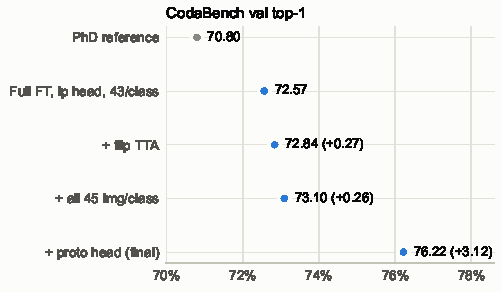
\includegraphics[width=\linewidth]{figures/fig1_codabench_progression_col.pdf}
  \caption{\textbf{CodaBench validation accuracy as we change one setting at a time} (all runs: full fine-tuning, 8 epochs). The gray dot is the reference. Positions encode values, so the axis starts at 70\%.}
  \label{fig:progression}
\end{figure}

\section{Ablation tables}
\label{sec:ablation-tables}

\Cref{tab:peft,tab:length} give the numbers behind \cref{sec:ablation-peft,sec:ablation-length}.

\begin{table}[t]
  \centering
  \footnotesize
  \setlength{\tabcolsep}{3pt}
  \begin{tabular}{@{}lrrrrr@{}}
    \toprule
    LP head, 3 epochs & Params & Holdout & img/s & GB & ms \\
    \midrule
    LoRA qkv, lr $10^{-3}$ & 0.344\% & 68.57 & 1,341 & 13.5 & 7.22 \\
    LoRA qkv, lr $5{\times}10^{-4}$ & 0.344\% & 68.45 & 1,353 & 13.5 & 7.15 \\
    LoRA all linear & 1.375\% & \textbf{69.45} & 885 & 19.9 & 7.03 \\
    AdaptFormer & 1.387\% & 69.05 & 1,437 & 12.8 & 9.89 \\
    \midrule
    Full fine-tuning & 100\% & 70.88 & 1,131 & 18.9 & 7.31 \\
    \bottomrule
  \end{tabular}
  \caption{\textbf{PEFT design.} Params: trainable backbone parameters (head excluded). img/s: training throughput; GB: peak training memory; ms: batch-1 latency after merging (A100, bf16).}
  \label{tab:peft}
\end{table}

\begin{table}[t]
  \centering
  \footnotesize
  \setlength{\tabcolsep}{3.5pt}
  \begin{tabular}{@{}lrrr@{}}
    \toprule
    Setting & Short (ep) & Long (ep) & $\Delta$ \\
    \midrule
    Full FT, LP & 70.88 (3) & 72.31 (8) & $+$1.43 \\
    Full FT, prototype, final$^\ddagger$ & 74.01 (3) & 76.22 (8) & $+$2.21 \\
    LoRA qkv, LP$^\dagger$ & 68.57 (3) & 68.69 (10) & $+$0.12 \\
    LoRA all, LP & 69.45 (3) & 69.87 (6) & $+$0.42 \\
    LoRA all, prototype & 71.98 (3) & 71.52 (6) & \minus0.46 \\
    \bottomrule
  \end{tabular}
  \caption{\textbf{Training length} (holdout top-1, \%; LoRA all: LoRA on all linear layers).
  $^\ddagger$All 45 images per class with flip TTA, CodaBench validation.
  $^\dagger$The 10-epoch run also lowered the head learning rate to $2{\times}10^{-4}$.}
  \label{tab:length}
\end{table}

\section{Hyperparameters}
\label{sec:hparams}

\begin{table}[h]
  \centering
  \scriptsize
  \renewcommand{\arraystretch}{1.05}
  \begin{tabular}{@{}p{2.2cm}p{3.5cm}p{3.5cm}p{3.5cm}p{3.0cm}@{}}
    \toprule
    & Full fine-tuning & LoRA & AdaptFormer & Linear-probe head \\
    \midrule
    Trainable & all weights + head & $A, B$ in qkv, proj, fc1, fc2 (all 12 blocks) + head & parallel MLP adapters + head & head only, on cached features \\
    Method-specific & layer-wise lr decay 0.75, drop path 0.1 & $r=8$, $\alpha=16$, no dropout, no layer decay, no drop path, merged after training & bottleneck 64, scale 0.1, dropout 0.1 & initialized from the prototype head \\
    Optimizer & AdamW & AdamW & AdamW & AdamW \\
    Learning rate & $10^{-4}$ (head $10^{-4}$) & $10^{-3}$ (head $10^{-3}$) & $10^{-3}$ (head $10^{-3}$) & $10^{-3}$ \\
    Weight decay & 0.05 & $10^{-4}$ & $10^{-4}$ & $10^{-4}$ \\
    Schedule & \multicolumn{3}{p{11.3cm}}{linear warmup (1 epoch; 0.3 epochs for 3-epoch runs), then cosine decay to 0} & cosine, no warmup \\
    Epochs & 3 or 8 & 3, 6 or 10 & 3 & 10 \\
    Batch size & 256 & 256 & 256 & 4,096 \\
    Precision & bf16 & bf16 & bf16 & fp32 head, fp16 features \\
    Regularization & \multicolumn{3}{p{11.3cm}}{label smoothing 0.1, gradient clipping at norm 1.0} & label smoothing 0.1 \\
    Augmentation & \multicolumn{3}{p{11.3cm}}{RandomResizedCrop (scale 0.25--1) + horizontal flip} & none (center crops) \\
    \bottomrule
  \end{tabular}
  \caption{\textbf{Hyperparameters.} Weight decay is not applied to biases, normalization parameters, the class token and position embeddings. Evaluation resizes to 248 pixels and takes a 224 center crop.}
  \label{tab:hparams}
\end{table}

Methods added for \cref{sec:compare} train for 3 epochs with the settings above, except: partial fine-tuning uses learning rate $3{\times}10^{-4}$ and weight decay 0.05 for $K = 1, 2$ and the full fine-tuning settings for $K = 4, 6$ (drop path only in trained blocks); BitFit uses learning rate $10^{-3}$ and no weight decay; the Adapter is AdaptFormer's bottleneck placed after the MLP, with scale 1.0.
